\documentclass[a4paper]{article} % formato de plantilla a utilizar

\usepackage[utf8]{inputenc}
\usepackage[spanish]{babel}
\usepackage[margin=2cm,top=2cm,includefoot]{geometry}
\usepackage{graphicx} % Para la inserción de imágenes
\usepackage[table, xcdraw]{xcolor} % PAra la inclusión de colores
\usepackage[T1]{fontenc}
\usepackage[most]{tcolorbox} % Para la inserción de cuadros en la portada
\usepackage{fancyhdr} % Definir el estilo de la página
\usepackage[hidelinks]{hyperref} % Libreria de hipervinculos
\usepackage{listings} % Para la inserción de codigo del documento
\usepackage{parskip} % Arreglo de taulaciones
\usepackage[figurename=Imagen]{caption} % Como nombrar a las imágenes
\usepackage{smartdiagram} % Para la inserción de diagramas
\usepackage{zed-csp} % Para la inserción de esquemas

% Declaración de colores
\definecolor{greeenPortada}{HTML}{69A84F}

% Declaración de variables
\newcommand{\logoPortada}{logo_htb.png}
\newcommand{\machineName}{Mantis} % Nombre de la máquina
\newcommand{\logoMachine}{mantis_logo.png} % Logo de la máquibna
\newcommand{\startDate}{18 de Juunio de 2022} % Fecha de Inicio de la auditoria

% Addicionales
\addto\captionsspanish{\renewcommand{\contentsname}{Indice}} % Camnio del titulo del indice
\setlength{\headheight}{40.2pt}
\pagestyle{fancy}
\fancyhf{}
\lhead{\includegraphics[width=5cm]{\logoPortada}}
\rhead{\includegraphics[height=1.5cm]{\logoMachine}}
\renewcommand{\headrulewidth}{3pt}
\renewcommand{\headrule}{\hbox to\headwidth{\color{greeenPortada}\leaders\hrule height \headrulewidth\hfill}}
\renewcommand{\lstlistingname}{Código}

\definecolor{codegreen}{rgb}{0,0.6,0}
\definecolor{codegray}{rgb}{0.5,0.5,0.5}
\definecolor{codepurple}{rgb}{0.58,0,0.82}
\definecolor{backcolour}{rgb}{0.95,0.95,0.92}

\lstdefinestyle{mystyle}{
    backgroundcolor=\color{backcolour},   
    commentstyle=\color{codegreen},
    keywordstyle=\color{magenta},
    numberstyle=\tiny\color{codegray},
    stringstyle=\color{codepurple},
    basicstyle=\ttfamily\footnotesize,
    breakatwhitespace=false,         
    breaklines=true,                 
    captionpos=b,                    
    keepspaces=true,                 
    numbers=left,                    
    numbersep=5pt,                  
    showspaces=false,                
    showstringspaces=false,
    showtabs=false,                  
    tabsize=2
}

\lstset{style=mystyle}




% Comienzo del documento

\begin{document}
    \cfoot{\thepage}
    %Creación de portada
    \begin{titlepage}
    \centering
    \includegraphics[width=0.6\textwidth]{\logoPortada}\par\vspace{1cm}
    {\scshape\LARGE \textbf{Informe Técnico}\par}
    \vspace{0.2cm}
    {\Huge\bfseries\textcolor{greeenPortada}{Máquina \machineName}\par}
    \vfill\vfill
    \includegraphics[width=\textwidth,height=10cm,keepaspectratio]{\logoMachine}\par\vspace{1cm}
    \vfill
    \begin{tcolorbox}[colback=red!5!white,colframe=red!75!black]
        \centering
        Este docunento es confidencial y contiene información sensible.
        \\No debería ser imnpreso o compartido con terceras entidades.
    \end{tcolorbox}
    \vfill
    {\large \startDate\par}
    \vfill
    \end{titlepage}
    % ------------------------------------------------------------------
    % comienzo del TOC
    \clearpage
    \tableofcontents
    \clearpage
    % ------------------------------------------------------------------
    \section{Antecedentes}El presente documento recoge los 
    resultados obtenidos durante la fase de auditoría de la 
    maquina {\textbf\machineName} de la plataforma 
    \href{http://www.hackthebox.com}{\textbf{\color{blue}HackTheBox}}.
    \vspace{0.2cm}
    \begin{figure}[h]
    \centering
    
\includegraphics[width=\textwidth]{mantis.jpeg}
    \caption{Detalles de la maquina}
    \end{figure}
    \vspace{0.2cm}
    \begin{tcolorbox}[enhanced,attach boxed title to top center={yshift=-3mm,yshifttext=-1mm},
        colback=blue!5!white,colframe=blue!75!black,colbacktitle=greeenPortada!80!black,
        title=Dirección URL,fonttitle=\bfseries,
        boxed title style={size=small,colframe=red!50!black} ]
        \centering
        \href{https://hackthebox.es/home/machines/profile/98}{\color{blue}{https://hackthebox.es/home/machines/profile/98}}
    \end{tcolorbox}
    
    \section{Objetivos}
    Conocer el estado de seguridad del servidor \textbf{\machineName}, 
    enumerando posibles vectores de explotyación y determinando el alcance 
    e impacto que un atacante podría ocasionar sobre el sistema en producción.

    \subsection{Consideraciones}
    Una vez finalizadas las jornadas de auditoría, se llevará a cabo
    una fase de saneamientos y buenas practicas con el objetivo de 
    securizar el servidor y evitar ser víctimas de un futuro ataque 
    en base a los vectores explotados.
    
    \begin{figure}[h]
    \begin{center}
    \smartdiagram[priority descriptive diagram]{
        Reconocimiento sobre el sistema,
        Detección de vulnerabilidades,
        Explotación de vulnerabilidades,
        Securización del sistema
    }
    \end{center}    
    \caption{Flujo de trabajo}
    \end{figure}

    \clearpage
    \section{Análisi de vulnerabilidades}
    \subsection{Reconocimiento inicial}
    \vspace{0.2cm}

    Se comenzó realizando un analisis inicial sobre el sistema, 
    verificando que el sistema objetivo se encontrara accesible 
    desde el segmento de red en el que se opera.

    \begin{figure}[h]
    \begin{center}
    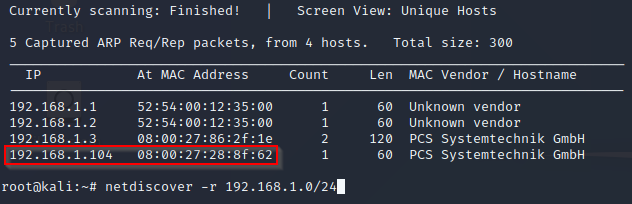
\includegraphics[width=0.8\textwidth]{newt_discover.png}
    \end{center}
    \caption{Reconocimiento inicial sobre el sistema objetivo}    
    \end{figure}

    \vspace{0.2cm}

    Una vez localizado se realizó un escaneo nmap a traves  
    de la herramienta \textbf{nmap} para la detección de 
    puertos abiertos, obteniendo los siguientes resultados:

    \begin{figure}[h]
    \begin{center}
    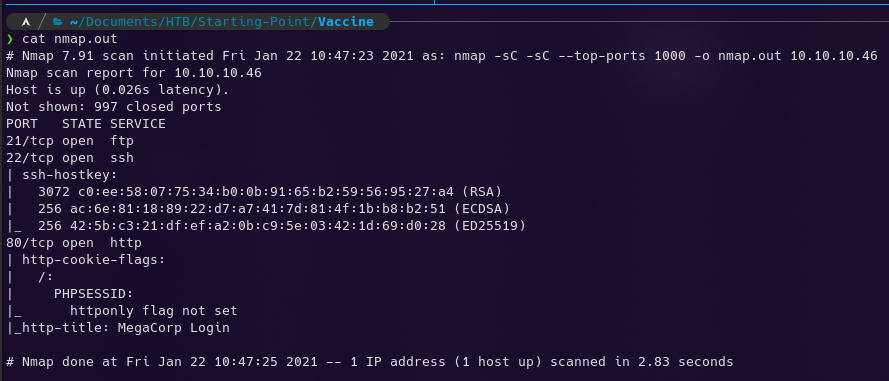
\includegraphics[width=\textwidth]{initial_recon.png}
    \end{center}
    \caption{Reconocimiento inicial sobre el sistema objetivo}    
    \end{figure}

    \clearpage
    Asimismo, con el objetivo de evitar falsos positivos, se diseñó 
    un script en \textbf{Bash} para enumerar  posibles puertos 
    adiccionales que la herramienta nmap no llegara a detectar:

    \vspace{0.2cm}

    \begin{lstlisting}[language=Bash, caption=Script personalizado para la enumeración de puertos]
    #!/bin/Bash

    for port in $(seq 1 65535); do
        timeout 1 bash -c "echo > /dev/tcp/10.10.10.52/$port" > /dev/null && echo "$port/tcp" &
    done; wait
        
    \end{lstlisting}
    
    \vspace{0.3cm}

    A través de este script, fue posible detectar puertos addiconalmente 
    abiertos:

    \begin{schema}{TCP}
    Puertos
    \where
    593, 1337
    \end{schema}

    Una vez finalizada la fase de enumertación de puertos, se 
    detectaron los servicios y versiones que corrian bajo estos, 
    representando a continuación los mas significativos bajo los 
    cuales fue posiblñe explotar el sistema:

    \begin{figure}[h]
    \centering
    \makebox[\textwidth]{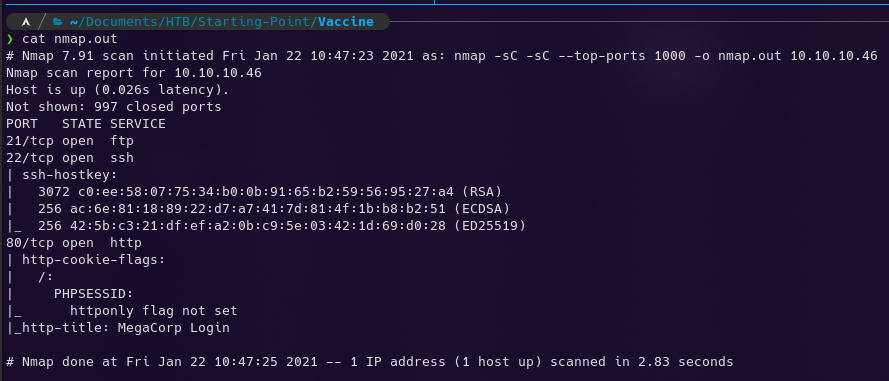
\includegraphics[width=0.9\paperwidth]{initial_recon.png}}
    \caption{Enumeración de servicios y versiones}    
    \label{fig:servicesResults}
    \end{figure}

    \vspace{0.2cm}

    Tal y como se aprecia en la figura \ref{fig:servicesResults} de la 
    página \pageref{fig:servicesResults} es posible identificar  que se 
    trata de una máquina con \textbf{Directorio Activo} configurado.

\end{document}

